\documentclass{article}
\usepackage[utf8]{inputenc}

\usepackage[framed,numbered,autolinebreaks,useliterate]{mcode}
\usepackage{url}
\setlength{\parindent}{0pt}
\setlength{\parskip}{18pt}

\usepackage{graphicx}

\title{\textbf{Numerical Analysis – Winter 2021}}
\author{\textbf{3180100675}}
\date{2021.11.25}

\begin{document}

\maketitle

\section{Problem 1:}  

\subsection{a}
Assume $f(x_1)<=f(x_2)$, so $f(x_1)\le \frac{f(x_1)+f(x_2))}{2}\le f(x_2)$, refer to “Intermediate Value Theorem”, there must be a $\xi$ between $(x_1,x_2)$, that fits $f(\xi)=\frac{f(x_1)+f(x_2)}{2}$. When the condition is reverse, we can proof it in the same way!

\subsection{b}
Assume $f(x_1)<=f(x_2)$, so $f(x_1)=\frac{c_1\times f(x_1)+c_2\times f(x_1)}{c_1+c_2}\le \frac{c_1\times f(x_1)+c_2\times f(x_2)}{c_1+c_2}\le \frac{c_1\times f(x_2)+c_2\times f(x_2)}{c_1+c_2}=f(x_2)$, refer to “Intermediate Value Theorem”, there must be a $\xi$ between $(x_1,x_2)$, that fits $f(\xi)=\frac{c_1\times f(x_2)+c_2\times f(x_2)}{c_1+c_2}$. When the condition is reverse, we can proof it in the same way!

\subsection{c}
Given $f(x)=x$, and $c_1=2$, $c_2=-1$, $(x_1,x_2)=(0,1)$ there is no $\xi$ that fits $f(\xi)=\frac{2\times f(0)-f(1)}{2-1}=-1$, for $f(x)\in (0,1)$.

\section{Problem 2:}
\subsection{a}
Absolute error= $|f(x_0)-f\tilde(x_o)|=|f(x_0)-f(x_0+\epsilon)|=|f^{'}(c)\epsilon|$ where $c\in (x_0,x_o+\epsilon)$.
And relative error = $\frac{|f^{'}(c)\epsilon|}{|f(x_0)|}$, and $c\in (x_0,x_0+\epsilon)$.

\subsection{b}
Refer to a, it is easy to get:
\subsubsection{\romannumeral1}
Absolute error$\le |{f^{'}(1+5\times 10^{-6})\times 5\times 10^{-6}}|=1.36\times 10^{-5}$; \\
Relative error$\le \frac{|{f^{'}(1+5\times 10^{-6})\times 5\times 10^{-6}}|}{|f(1)|}=0.50\times 10^{-5}$
\subsubsection{\romannumeral2}
Absolute error$\le |{f^{'}(1)\times 5\times 10^{-6}}|=0.27\times 10^{-5}$;\\
Relative error$\le \frac{|{f^{'}(1)\times 5\times 10^{-6}}|}{|f(1)|}=0.32\times 10^{-5}$

\subsection{c}
\subsubsection{\romannumeral1}
Absolute error$\le |{f^{'}(10+5\times 10^{-5})\times 5\times 10^{-5}}|=1.10$; \\
Relative error$\le \frac{|{f^{'}(10+5\times 10^{-5})\times 5\times 10^{-5}}|}{|f(10)|}=0.50\times 10^{-4}$
\subsubsection{\romannumeral2}
Absolute error$\le |{f^{'}(10)\times 5\times 10^{-5}}|=0.42\times 10^{-4}$;\\
Relative error$\le \frac{|{f^{'}(10)\times 5\times 10^{-5}}|}{|f(10)|}=0.79\times 10^{-4}$

\section{Problem 3:}
\subsection{\romannumeral1}
a. $\frac{4}{5}+\frac{1}{3}=\frac{17}{15}=1.1333\.{3}$ \\
b. $(\frac{1}{3}+\frac{3}{11})-\frac{3}{20}=\frac{301}{660}=0.456\.{0}\.{6}$
\subsection{\romannumeral2}
a. $\frac{4}{5}+\frac{1}{3}=1.13$ \\
b. $(\frac{1}{3}+\frac{3}{11})-\frac{3}{20}=0.456$
\subsection{\romannumeral3}
a. $\frac{4}{5}+\frac{1}{3}=1.13$ \\
b. $(\frac{1}{3}+\frac{3}{11})-\frac{3}{20}=0.456$
\subsection{\romannumeral4}
Their results are same, so i just compute one of them: \\
a. relative error=$|\frac{(\frac{4}{5}+\frac{1}{3}-1.13)}{\frac{4}{5}+\frac{1}{3}}=0.294$\%$ $ \\
b. relative error=$|\frac{(\frac{1}{3}+\frac{3}{11})-\frac{3}{20}-0.456}{(\frac{1}{3}+\frac{3}{11})-\frac{3}{20}}|=0.0133$\%$ $

\section{Problem 4:}   
To proof this problem, i just need to proof that: \\
$O(x^{\alpha})+O(x^{\beta})=O(x^{\gamma})$; \\
and refer to Page25 in "Lec01.pdf", the largest value $p>0$ such that $\alpha_n=\alpha+O(\frac{1}{n^{p}})$, so $O(x^{\alpha})+O(x^{\beta})=O(x^{min(\alpha,\beta)})=O(x^{\gamma})$ \\
Then it is easy to draw below conclusions:
\subsection{a}
$F(x)=c_1 F_1(x)+c_2 F_2(x) \\
=c_1 L_1+c_2 L_2+c_1 O(x^{\alpha})+c_2 O(x^{\beta}) \\
=c_1 L_1+c_2 L_2+O(x^{\gamma})$
\subsection{b}
$G(x)=F_1(c_1 x)+F_2(c_2 x) \\
=L_1+L_2+O((c_1 x)^{\alpha})+O((c_2 x)^{\beta}) \\
=L_1+L_2+O(x^{\gamma})$

\section{Problem 5:}
Appendix A is the Bisection Algorithm, and for these two equation, their roots are: \\
a. root = 0.257530; \\

\begin{figure}[htbp]
\centering
\subfigure{
\begin{minipage}[t]{0.3\linewidth}
\centering
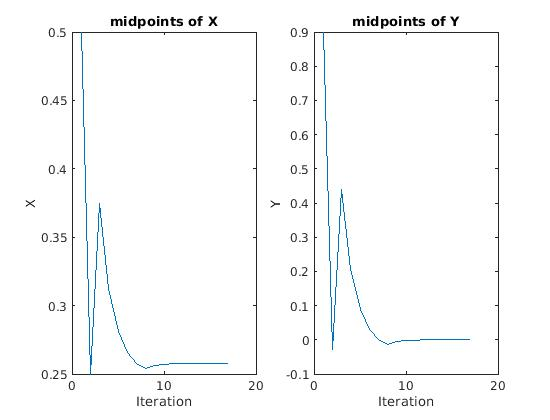
\includegraphics[width=2.75cm]{P5-func1-0.25.jpg}
\caption{-0.45}
\end{minipage}%
}%
% \caption{midpoints}
\end{figure}


b. root1 = 0.297528, root2 = 1.256622;
\begin{figure}[htbp]
\centering
\subfigure{
\begin{minipage}[t]{0.3\linewidth}
\centering
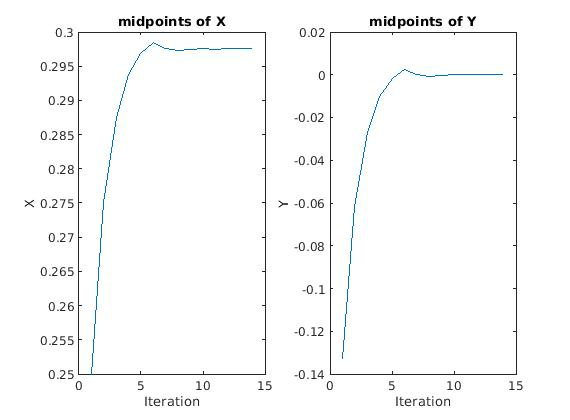
\includegraphics[width=2.75cm]{P5-func2-0.29.jpg}
\caption{-0.45}
\end{minipage}%
}%
\subfigure{
\begin{minipage}[t]{0.3\linewidth}
\centering
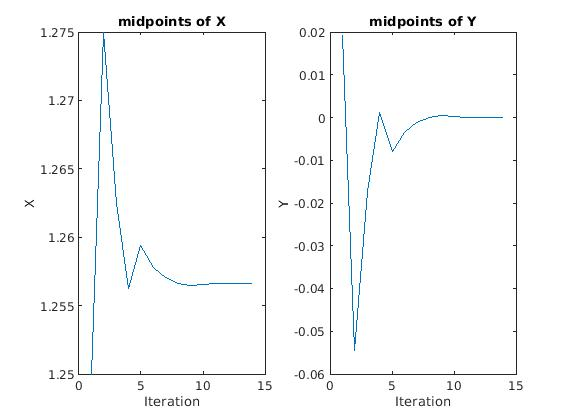
\includegraphics[width=2.75cm]{P5-func2-1.25.jpg}
\caption{0.91}
\end{minipage}%
}%
% \caption{midpoints}
\end{figure}

\section{Problem 6:} 
Appendix B is the Fixed Point Algorithm, and for these two equation, their roots are: \\
a. root =  1.206023 or 1.681972; \\
\begin{figure}[htbp]
\centering
\subfigure{
\begin{minipage}[t]{0.3\linewidth}
\centering
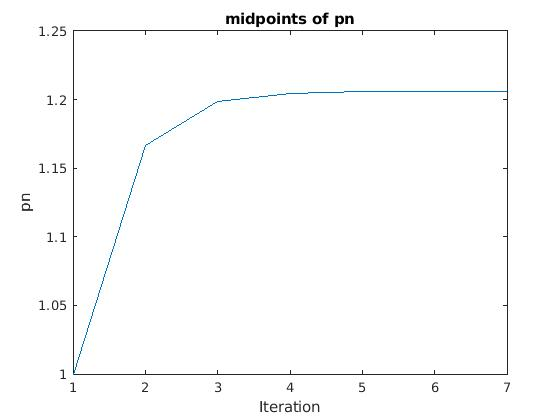
\includegraphics[width=2.75cm]{P6-func1-1.20.jpg}
\caption{-0.45}
\end{minipage}%
}%
\subfigure{
\begin{minipage}[t]{0.3\linewidth}
\centering
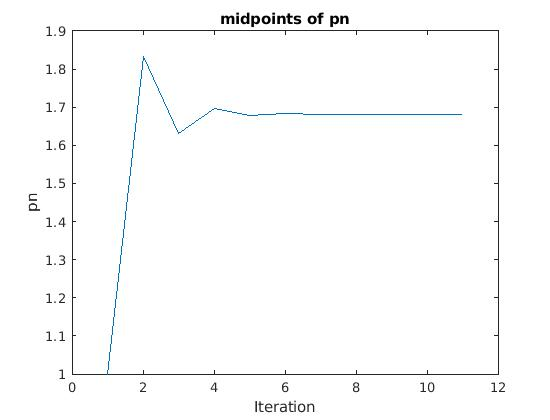
\includegraphics[width=2.75cm]{P6-func1-1.68.jpg}
\caption{0.91}
\end{minipage}%
}%
% \caption{midpoints}
\end{figure}

b. root1 = -0.458966, root2 = 0.910010, root3 = 3.733066;
\begin{figure}[htbp]
\centering
\subfigure{
\begin{minipage}[t]{0.3\linewidth}
\centering
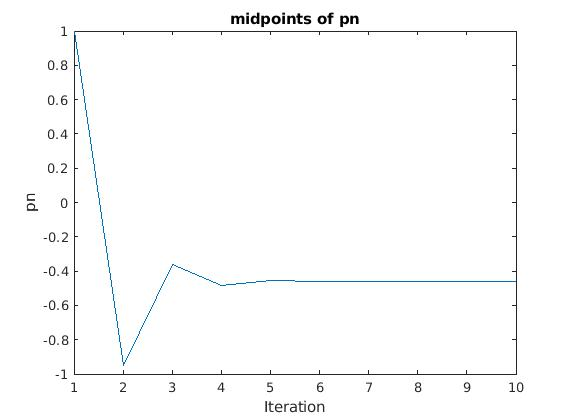
\includegraphics[width=2.75cm]{P6-func2--0.45.jpg}
\caption{-0.45}
\end{minipage}%
}%
\subfigure{
\begin{minipage}[t]{0.3\linewidth}
\centering
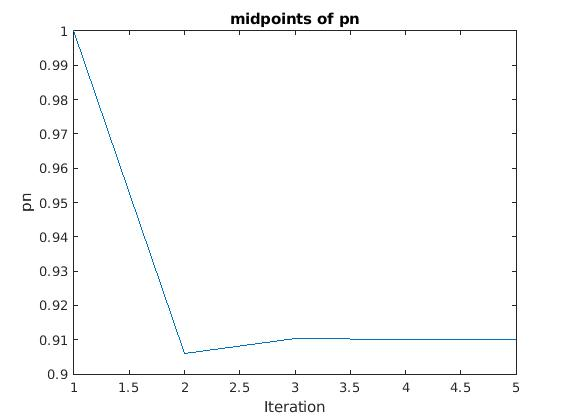
\includegraphics[width=2.75cm]{P6-func2-0.91.jpg}
\caption{0.91}
\end{minipage}%
}%
\subfigure{
\begin{minipage}[t]{0.3\linewidth}
\centering
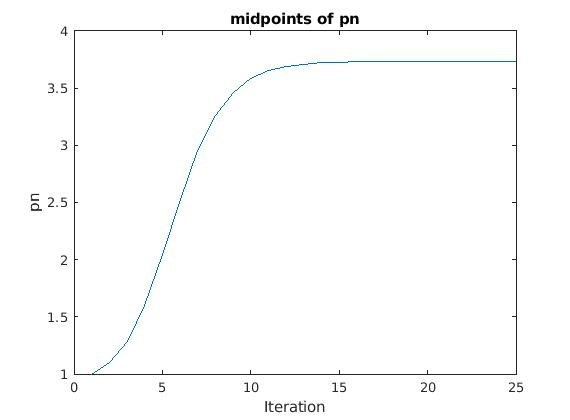
\includegraphics[width=2.75cm]{P6-func2-3.73.jpg}
\caption{3.73}
\end{minipage}
}%
% \caption{midpoints}
\end{figure}
	 

\section{Problem 7:}     
Due to $p_0=p+\delta$, $p_1=g(p_0)=g(p+\delta)$; \\
Apply "Taylor Expansion", and discard high-order infinitesimals, then: \\
$p_1=g(p)+g^{'}(p)\times \delta+...$; \\
so $|p_1-p|=|g(p)+g^{'}(p)\times \delta+...-p| \\
=|g^{'}(p)\times \delta+...| \\
\approx |g^{'}(p)\times \delta|\\
>|\delta| \\
>|p_0-p|$

\newpage
\appendix
\section{Appendix A}

\begin{lstlisting}
clear; clc; close all;
%% Main process
Bisection(0, 1, @func1);
Bisection(0.2, 0.3, @func2);
Bisection(1.2, 1.3, @func2);

%% Bisection
function Bisection(left, right, f)
    i = 1;
    MaxIteration = 100;
    Tolerance = 10 ^ -5;
    xList = [];
    yList = [];
    currX = (left + right) / 2;
    currY = f(currX);
    for i = 1 : MaxIteration
        fprintf("[No.%d Iteration]: f(%f) = %f\n", i, currX, currY);
        xList(i) = currX;
        yList(i) = currY;
        
        if abs(currY) < Tolerance
            fprintf("It costs me %d iterations to find the root\n", i);
            break;
        end
        if currY / f(left) > 0
            left = currX;
        else
            right = currX;
        end
        currX = (left + right) / 2;
        currY = f(currX);
    end
    fprintf("Final root is %f, and f(%f) = %f\n", currX, currX, currY);
    figure();
    subplot(1,2,1);
    plot(xList);title("midpoints of X");xlabel("Iteration");ylabel("X");
    subplot(1,2,2);
    plot(yList);title("midpoints of Y");xlabel("Iteration");ylabel("Y");
end
    
%% Mathmatic function
function y = func1(x)
    y = exp(x) - x ^ 2 + 3 * x - 2;
end

function y = func2(x)
    y = x * cos(x) - 2 * x ^ 2 + 3 * x - 1;
end
\end{lstlisting}

\section{Appendix B}
\begin{lstlisting}
clear; clc; close all;
%% Initialization
global formula; % Used to choose different type of g(x)
%% Main process
formula = 1; FixedPoint(1, @func1);
formula = 2; FixedPoint(1, @func1);
formula = 1; FixedPoint(1, @func2);
formula = 2; FixedPoint(1, @func2);
formula = 3; FixedPoint(1, @func2);
%% Fixed Point
function FixedPoint(p0, g)
    i = 1;
    MaxIteration = 100;
    Tolerance = 10 ^ -5;
    pList = [];
    newP = g(p0);
    for i = 1 : MaxIteration
        pList(i) = p0;
        fprintf("[No.%d Iteration]: pn = %f\n", i, newP);
        if abs(newP - p0) < Tolerance
            pList(i) = newP;
            fprintf("It costs me %d iterations to find the root\n", i);
            break;
        end
        p0 = newP;
        newP = g(p0);
    end
    fprintf("Final root is %f, and g(%f) = %f\n", newP, p0, newP);
    figure();
    plot(pList);title("midpoints of pn");xlabel("Iteration");ylabel("pn");
end
%% Mathmatic function
function y = func1(x) % 2 * sin(pi * x) + x; 
    global formula;
    if formula == 1
        y = 1 + asin(x / 2) / pi;% 1.206
    elseif formula == 2
        y = 2 + asin(-x / 2) / pi; % 1.681
    end
end
function y = func2(x) % 3 * x ^ 2 - exp(x);
    global formula;
    if formula == 1
        y = -(exp(x) / 3) ^ 0.5; % -0.45
    elseif formula == 2
        y = exp(x) / 3 / x; % 0.91
    elseif formula == 3 
        y = log(3 * x ^ 2); % 3.73
    end
end
\end{lstlisting}

\end{document}

